\chapter{Problem Statement}

Per risolvere il problema dell'Autonomous Driving (AU) di un veicolo terrestre, esso, normalmente, viene scomposto in diversi sotto problemi, ognuno dei quali viene risolto da uno specifico processo. Ad esempio, l'\textit{Obstacle Avoidance} è il processo che risolve la gestione degli ostacoli presenti sul percorso durante la guida, oppure l'\textit{Overtaking} è quello che si occupa di gestire il sorpasso di altri veicoli.
\newline

Tutti questi processi, però, fondano il loro corretto funzionamento sul fatto che, in principio, l'auto si trovi correttamente in carreggiata durante tutto il processo di guida. Il processo che risolve questo fondamentale problema viene detto \textit{Lane Keeping}.
\newline

I tradizionali sistemi di AU sono basati su regole precostruite e devono creare informazioni sulla struttura dalle scene prima di prendere una decisione. Le informazioni sulla struttura sono molto complicate, il che porta alla costruzione di regole complesse e quindi ad una difficile costruzione di un modello decisionale completo ed efficace.
Con gli ultimi sviluppi dell'Intelligenza Artificiale nell'AU è stato possibile affidare la comprensione di scene complesse e il processo decisionale alle reti neurali senza bisogno di regole definite dall'uomo. In queste circostanze è comune parlare di sistema decisionale end-to-end\footnote{Un sistema che produce una decisione direttamente a partire dalla comprensione dell'ambiente, senza passaggi intermedi.}.
\newline

L'obiettivo di questa tesi è quello di affrontare il problema del lane keeping nell'ambiente avanzato di simulazione di guida TORCS\cite{torcsWebsite}, attraverso un sistema decisionale end-to-end basato sul DDPG. Il lavoro si ispira a quello dei ricercatori della \textit{Beijing University of Technology}\cite{mainTORCSPaper}.


\section{Introduzione a TORCS}

TORCS\cite{torcsWebsite} è un simulatore 3D di gare automobilistiche open source. Esso è progettato per permettere a delle IA pre-programmate di gareggiare le une contro le altre e permette ad un giocatore di utilizzare una tastiera, un mouse, o un volante per controllare un veicolo.

\begin{figure}[hb]
    \centering
    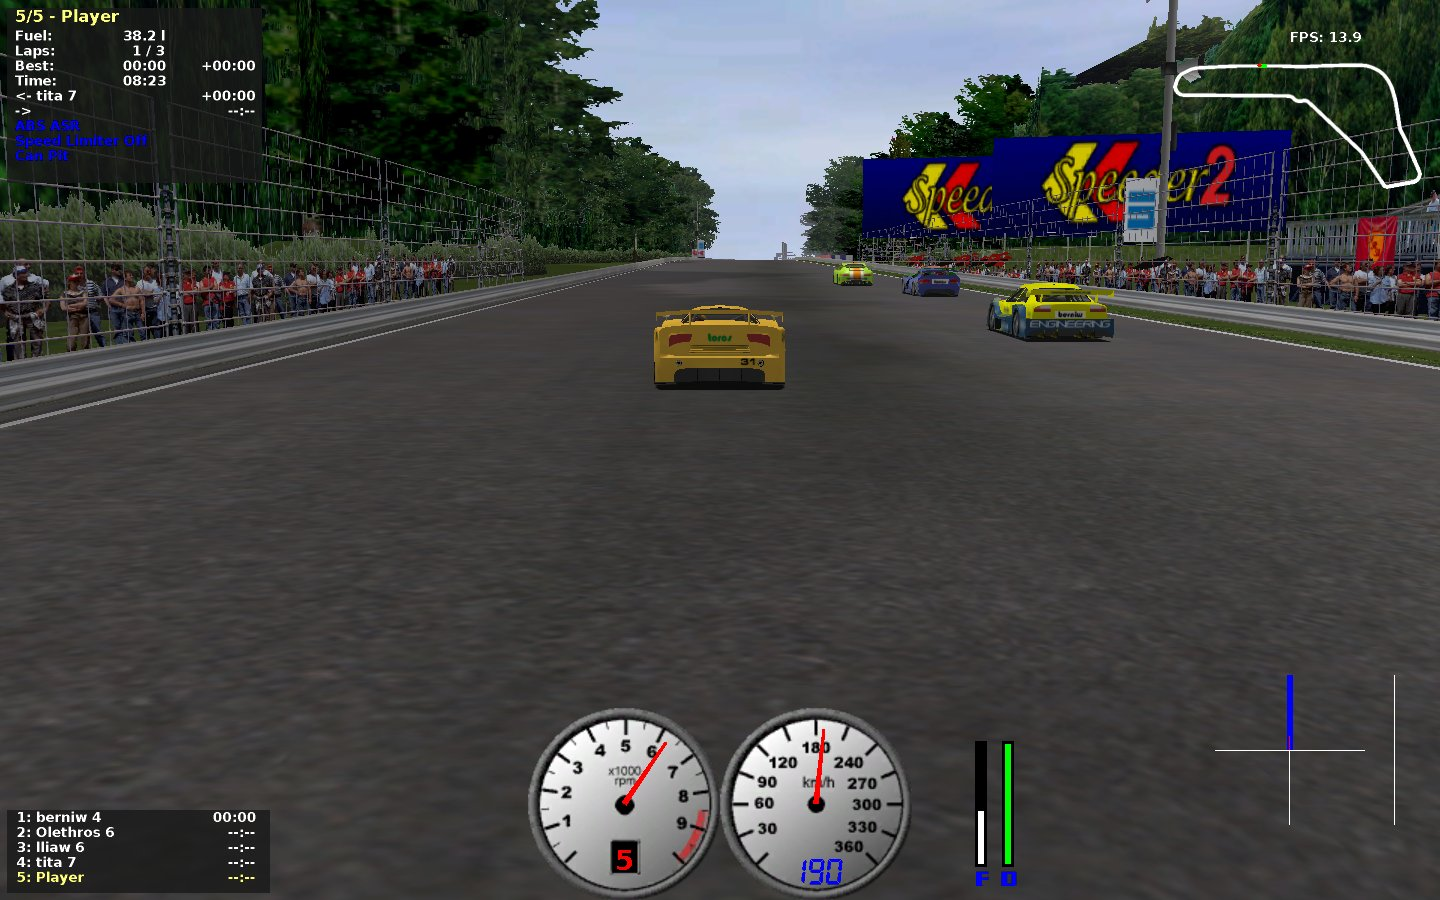
\includegraphics[width = 5in]{Figures/Chapter3/torcs_game.jpg}
    \caption{Immagine di una gara in TORCS}
    \label{fig:torcsgame}
\end{figure}

TORCS si presenta come un'applicazione autonoma in cui i bot vengono compilati come moduli separati che vengono caricati nella memoria principale quando si svolge una gara. Questo presenta diversi svantaggi sul profilo della realizzazione in quanto impone la modalità di interfacciamento col gioco e il linguaggio di programmazione da utilizzare.
\newline

Nell'ambito di questa tesi si è utilizzata la versione di TORCS con patch SCR.
\newline

Simulated Car Racing (SCR)\cite{scrloiaconoPaper} estende l'architettura TORCS originale sotto tre aspetti. Innanzitutto struttura TORCS come un'applicazione Client-Server: i bot vengono eseguiti come processi esterni connessi al server di gara tramite connessioni UDP. 

In secondo luogo, aggiunge il real-time: ad ogni tic di gioco (corrispondente all'incirca a 20 ms di tempo simulato), il server invia gli input sensoriali correnti a ciascun bot
e poi attende 10ms (di tempo reale) per ricevere un'azione dal bot. Se non arriva nessuna azione la simulazione continua e viene utilizzata l'ultima azione eseguita. 

Infine SCR costruisce un livello d'astrazione che garantisce una separazione fisica tra il codice dell'AI di guida  e il server di gara, \textit{un modello di sensori e attuatori}, che lascia completa libertà di scelta in merito al linguaggio di programmazione utilizzato per i bot.
\newline

Nella figura seguente viene mostrata l'architettura di SCR.

\begin{figure}[hb]
    \centering
    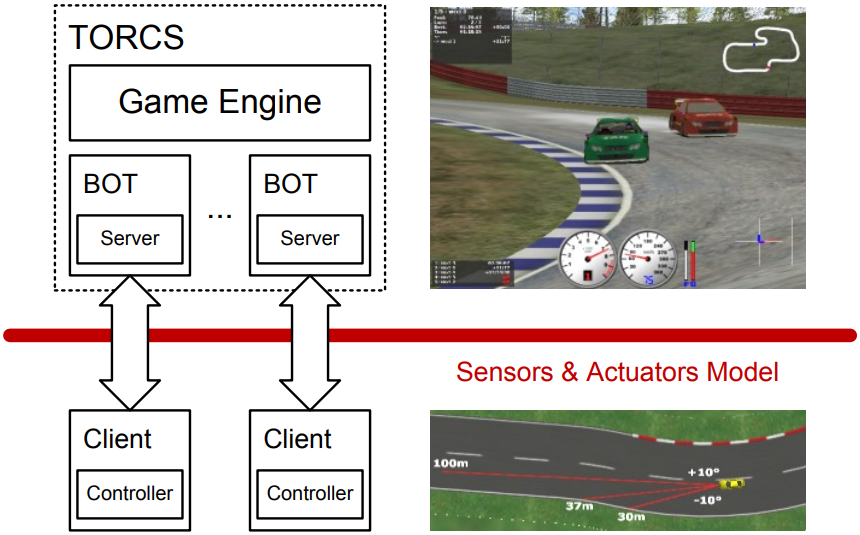
\includegraphics[width = 4in]{Figures/Chapter3/scr_model.png}
    \caption{Architettura di SCR}
    \label{fig:scrmodel}
\end{figure}

La lista completa dei sensori e degli attuatori forniti da SCR non è riportata per brevità ma è consultabile in\cite{scrloiaconoPaper}.

\clearpage

\section{Segnali di interazione con l'ambiente}

In questo lavoro si presenta un agente capace di terminare il percorso di gara, rimanendo sempre in carreggiata, utilizzando un sottoinsieme dei sensori forniti da TORCS. Nella tab.\ref{tab:statetable} sono definiti i sensori utilizzati per costruire lo stato $s$ mentre nella tab.\ref{tab:actiontable} gli attuatori, ovvero l'azione $a$ che l'agente può eseguire sull'ambiente.

\begin{table}[hb]
\centering
\begin{tabular}{|ccl|}
\hline
\multicolumn{1}{|l|}{{\color[HTML]{000000} \textbf{Nome}}} &
  \multicolumn{1}{c|}{{\color[HTML]{000000} \textbf{Range (unità)}}} &
  \multicolumn{1}{c|}{{\color[HTML]{000000} \textbf{Descrizione}}} \\ \hline
\multicolumn{1}{|c|}{{\color[HTML]{000000} angle}} &
  \multicolumn{1}{c|}{{\color[HTML]{000000} $[-\pi,+\pi] (rad) \in \mathbb{R}$}} &
  {\color[HTML]{000000} \begin{tabular}[c]{@{}l@{}}Angolo tra la direzione dell'auto \\ e l'asse della carreggiata\end{tabular}} \\ \hline
\multicolumn{1}{|c|}{{\color[HTML]{000000} speedX}} &
  \multicolumn{1}{c|}{{\color[HTML]{000000} $[0,300] (km/h) \in \mathbb{R}$}} &
  {\color[HTML]{000000} \begin{tabular}[c]{@{}l@{}}Velocità dell'auto lungo il suo asse longitudinale\end{tabular}} \\ \hline
\multicolumn{1}{|c|}{speedY} &
  \multicolumn{1}{c|}{$[0,300] (km/h) \in \mathbb{R}$} &
  \begin{tabular}[c]{@{}l@{}}Velocità dell'auto lungo il suo asse trasversale\end{tabular} \\ \hline
\multicolumn{1}{|c|}{speedZ} &
  \multicolumn{1}{c|}{$[0,300] (km/h) \in \mathbb{R}$} &
  \begin{tabular}[c]{@{}l@{}}Velocità dell'auto lungo il suo asse Z\end{tabular} \\ \hline
\multicolumn{1}{|c|}{track} &
  \multicolumn{1}{c|}{$[0,200] (m) \in \mathbb{R}^{19}$} &
  \begin{tabular}[c]{@{}l@{}}Vettore di 19 rangefinder disposti a diverse\\ angolazioni davanti l'auto: ogni sensore\\ misura la distanza tra l'auto e il bordo \\ della carreggiata in un range di 200 metri\end{tabular} \\ \hline
\multicolumn{1}{|c|}{trackPos} &
  \multicolumn{1}{c|}{$[-1,+1] \in \mathbb{R}$} &
  \begin{tabular}[c]{@{}l@{}}Distanza normalizzata tra l'auto \\ e l'asse della carreggiata\end{tabular} \\ \hline
\end{tabular}
\caption{Sensori utilizzati nella costruzione del vettore di stato}
\label{tab:statetable}
\end{table}


\begin{table}[hb]
\centering
\begin{tabular}{|ccl|}
\hline
\multicolumn{1}{|l|}{{\color[HTML]{000000} \textbf{Nome}}} &
  \multicolumn{1}{c|}{{\color[HTML]{000000} \textbf{Range (unità)}}} &
  \multicolumn{1}{c|}{{\color[HTML]{000000} \textbf{Descrizione}}} \\ \hline
\multicolumn{1}{|c|}{{\color[HTML]{000000} accel}} &
  \multicolumn{1}{c|}{{\color[HTML]{000000} $[0,1] \in \mathbb{R}$}} &
  {\color[HTML]{000000} \begin{tabular}[c]{@{}l@{}}Pedale del gas virtuale  (0 significa accelerazione\\ nulla e 1 accelerazione massima)\end{tabular}} \\ \hline
\multicolumn{1}{|c|}{{\color[HTML]{000000} brake}} &
  \multicolumn{1}{c|}{{\color[HTML]{000000} $[0,1] \in \mathbb{R}$}} &
  {\color[HTML]{000000} \begin{tabular}[c]{@{}l@{}}Pedale del freno virtuale (0 significa frenata\\ nulla e 1 frenata massima)\end{tabular}} \\ \hline
\multicolumn{1}{|c|}{steer} &
  \multicolumn{1}{c|}{$[-1,+1] \in \mathbb{R}$} &
  \begin{tabular}[c]{@{}l@{}}Sterzo virtuale (-1 significa sterzata massima\\ a destra e +1 sterzata massima a sinistra)\\ Sterzata massima di $0,366519 \, rad$\end{tabular} \\ \hline
\end{tabular}
\caption{Azioni eseguibili dall'agente}
\label{tab:actiontable}
\end{table}

Nella modellazione si è scelto di direzionare i 19 rangefinder nelle seguenti angolazioni: (-45, -19, -12, -7, -4, -2.5, -1.7, -1, -0.5, 0, 0.5 , 1, 1.7, 2.5, 4, 7, 12, 19, 45) gradi. In definitiva lo spazio di stato dell'agente è $s \in \mathbb{R}^{24}$ e quello di azione è $a \in \mathbb{R}^{3}$.

\clearpage